\documentclass[12pt]{article}
\usepackage{natbib}
\usepackage{url}
\usepackage{stmaryrd}
\usepackage{mathrsfs}
\usepackage{amsmath}
\usepackage{graphicx}
\usepackage{parskip}
\usepackage{fancyhdr}
\usepackage{commath}%定义d
\usepackage[UTF8,scheme = plain]{ctex}
\usepackage{geometry}
\usepackage{bm}
\usepackage{siunitx}
\usepackage{float}
\usepackage{subfig}
\usepackage{titlesec}
\usepackage{caption}
\usepackage{paralist}
\usepackage{multirow}
\usepackage{booktabs} % To thicken table lines
\usepackage{diagbox}
\usepackage{authblk}
\usepackage{indentfirst}
\usepackage{amsthm}
\usepackage{fontspec}
\usepackage{color}
%\usepackage{txfonts} %设置字体为times new roman
\usepackage{lettrine}
\usepackage{nameref}
%\usepackage[nottoc]{tocbibind}
\usepackage{amssymb}%font
\usepackage{lipsum}%make test words
\usepackage{picinpar}%words around the picture
\usepackage[all]{xy}%draw arrow
\usepackage{asymptote}%draw picture
\usepackage[perpage]{footmisc}%脚注每页清零
\usepackage{esint}

\geometry{bottom=3cm,left=3cm,right=3cm,top=3cm}
% \footskip = 60pt

% \setmainfont{TimesNewRomanPSMT}
\setsansfont{Helvetica-Light}
\setCJKmainfont[ItalicFont=STKaitiSC-Regular,BoldFont=STSongti-SC-Black]{STSongti-SC-Regular}
\setCJKsansfont[BoldFont=STHeitiSC-Medium]{STHeitiSC-Light}


%\setmainfont{Times New Roman}

\ctexset{today=old}%日期类型设置

% ======================================
% = Color de la Universidad de Sevilla =
% ======================================
\usepackage{tikz}
\definecolor{PKUred}{cmyk}{0,1,1,0.45}

%超链接设置
\usepackage[breaklinks,colorlinks,linkcolor=PKUred,citecolor=PKUred,pagebackref,urlcolor=PKUred]{hyperref}
\usepackage{cleveref}
% \newcommand{\crefpairconjunction}{ 和 }


\newcommand{\hsp}{\hspace{20pt}}
\newcommand{\nhsp}{\hspace{-30pt}}
\titleformat{\section}{\Large\bfseries}{%\arabic{section}
\hspace{-22pt}\textcolor{PKUred}{\vrule width 2pt}\hsp}{0pt}{}


\titleformat{\subsection}
  {\normalfont\large\bfseries}{}{0em}{}

\renewcommand*\footnoterule{%
    \vspace*{-3pt}%
    {\color{PKUred}\hrule width 2in height 0.4pt}%
    \vspace*{2.6pt}%
}


%% Color the bullets of the itemize environment and make the symbol of the third
%% level a diamond instead of an asterisk.
%h\renewcommand*\textbullet{\dag}
\renewcommand*\labelitemi{\color{PKUred}\textbullet}
\renewcommand*\labelitemii{\color{PKUred}--}
\renewcommand*\labelitemiii{\color{PKUred}$\diamond$}
\renewcommand*\labelitemiv{\color{PKUred}\textperiodcentered}



%%% Equation and float numbering
\numberwithin{equation}{section}		% Equationnumbering: section.eq#
\numberwithin{figure}{section}			% Figurenumbering: section.fig#
\numberwithin{table}{section}				% Tablenumbering: section.tab#


%代码设置
\usepackage{listings}
\usepackage{fontspec} % 定制字体
\newfontfamily\menlo{SFMono-Regular}
\usepackage{xcolor} % 定制颜色
\definecolor{mygreen}{rgb}{0,0.6,0}
\definecolor{mygray}{rgb}{0.5,0.5,0.5}
\definecolor{mymauve}{rgb}{0.58,0,0.82}
\lstset{  
numbers=left,
numberstyle=\footnotesize\menlo,
basicstyle=\footnotesize\menlo,
backgroundcolor=\color{white},      % choose the background color
columns=fullflexible,
tabsize=4,
breaklines=true,               % automatic line breaking only at whitespace
captionpos=b,                  % sets the caption-position to bottom
commentstyle=\color{mygreen},  % comment style
escapeinside={\%*}{*)},        % if you want to add LaTeX within your code
keywordstyle=\color{blue},     % keyword style
stringstyle=\color{mymauve}\ttfamily,  % string literal style
frame=single,
rulesepcolor=\color{red!20!green!20!blue!20},
% identifierstyle=\color{red},
language=c++,
xleftmargin=4em,xrightmargin=2em, aboveskip=1em,
framexleftmargin=2em,
numbers=left
}

%脚注
\renewcommand\thefootnote{\fnsymbol{footnote}}

%定义常数i、e、积分符号d
\newcommand\mi{\mathrm{i}}
\newcommand\me{\mathrm{e}}

%%% Maketitle metadata
\newcommand{\horrule}[1]{\rule{\linewidth}{#1}} 	% Horizontal rule
\newcommand{\tabincell}[2]{\begin{tabular}{@{}#1@{}}#2\end{tabular}}


\setcounter{secnumdepth}{2}
\usepackage{bm}
\usepackage{autobreak}
\usepackage{amsmath}
\graphicspath{{fig/}}

%pdf文件设置
\hypersetup{
	pdfauthor={袁磊祺},
	pdftitle={Advanced Fluid Mechanics Homework 1}
}

\title{
		\vspace{-1in} 	
		\usefont{OT1}{bch}{b}{n}
		\normalfont \normalsize \textsc{\LARGE Peking University}\\[1cm] % Name of your university/college \\ [25pt]
		\horrule{0.5pt} \\[0.5cm]
		\huge \bfseries{Advanced Fluid Mechanics Homework 1} \\
		\horrule{2pt} \\[0.5cm]
}
\author{
		\normalfont 								\normalsize
		College of Engineering \quad 2001111690  \quad 袁磊祺\\	\normalsize
        \today
}
\date{}

\begin{document}

% %%%%%%%%%%%%%%%%%%%%%%%%%%%%%%%%%%%%%%%%%%%%%%
\captionsetup[figure]{name={图},labelsep=period}
\captionsetup[table]{name={表},labelsep=period}
\renewcommand\contentsname{目录}
\renewcommand\listfigurename{插图目录}
\renewcommand\listtablename{表格目录}
\renewcommand\refname{参考文献}
\renewcommand\indexname{索引}
\renewcommand\figurename{图}
\renewcommand\tablename{表}
\renewcommand\abstractname{摘\quad 要}
\renewcommand\partname{部分}
\renewcommand\appendixname{附录}
\def\equationautorefname{式}%
\def\footnoteautorefname{脚注}%
\def\itemautorefname{项}%
\def\figureautorefname{图}%
\def\tableautorefname{表}%
\def\partautorefname{篇}%
\def\appendixautorefname{附录}%
\def\chapterautorefname{章}%
\def\sectionautorefname{节}%
\def\subsectionautorefname{小小节}%
\def\subsubsectionautorefname{subsubsection}%
\def\paragraphautorefname{段落}%
\def\subparagraphautorefname{子段落}%
\def\FancyVerbLineautorefname{行}%
\def\theoremautorefname{定理}%
\crefname{figure}{图}{图}
\crefname{equation}{式}{式}
\crefname{table}{表}{表}
%%%%%%%%%%%%%%%%%%%%%%%%%%%%%%%%%%%%%%%%%%%

\maketitle

\section{}

\subsection{}

The depth of the cylindrical buoy in the sea water is
\begin{equation}
	H = \frac{W}{\rho \times \frac{\pi}{4} D^2} = \frac{770}{1025 \times \frac{\pi}{4} \times 0.9^2} \mathrm{m} \approx 1.18 \mathrm{m},
\end{equation}
where $W$ is the weight of the cylinder, $\rho$ is the density of the sea water and $D$ is the diameter of the cylinder.

The distance between the floating center and the bottom is
\begin{equation}
	L_f = H/2 = 0.59 \mathrm{m},
\end{equation}
which is smaller than 0.9m. The floating center is higher than centroid of the cylinder, so the cylinder can't float upright stably.\qed

\subsection{}

To keep the cylinder upright stably by minimal force,
\begin{equation}
	W \left(H_c-\frac{H'}{2}\right) = \frac{H'}{2}F ,
\end{equation}
where $H_c$ is the height of the cylinder' centroid, $H'$ is the depth of immersion in water.

And to keep the cylinder balance,
\begin{equation}
		F = \left(\frac{\pi}{4}D^2\times H'\times \rho - W\right)
\end{equation}
So the minimal force we need is
\begin{equation}
	\begin{split}
		F \approx 656 \mathrm{kg}.
	\end{split}
\end{equation}

\section{}

The lift coefficient $C_L$ is defined by
\begin{equation}
	C_\mathrm{L} = \frac{L}{\frac{1}{2}\rho u^2 S},
\end{equation}
where  $L$ is the lift force,  $S$ is the relevant surface area and $q$ is the fluid dynamic pressure, in turn linked to the fluid density $\rho$.

The drag coefficient c dc d is defined as
\begin{equation}
	{ C_{\mathrm {d} }={\dfrac D{\frac{1}{2}\rho u^{2}S}}},
\end{equation}
D is the drag force, which is by definition the force component in the direction of the flow velocity.

During cruise the aircraft weight $w$ changes at a rate equal to g times the mass flow rate at which fuel is burned, that is
\begin{equation}
	\frac{\dif w}{\dif t} = - g \times \mathrm{sfc} \times D = - g \frac{\mathrm{sfc}\times w}{L/D},
\end{equation}
where $L/D$ is the ratio of lift to drag, sfc is specific fuel consumption (actually the thrust specific fuel consumption) equal to the mass flow rate of fuel divided by net thrust and we use $w \equiv L$. Rearranging
\begin{equation}
	\frac{\dif w}{w} = - g \frac{\mathrm{sfc}\times \dif t}{L/D}.
\end{equation}
This equation can then be rewritten in terms of the distance travelled $s$ as
\begin{equation}
	\frac{\dif w}{w} = - g \frac{\mathrm{sfc}\times \dif s}{uL/D}.
\end{equation}

An aircraft will obtain maximum range if it flies at a value of $uL/D$ which is close to the maximum; this quantity can be kept constant during the cruise by increasing altitude as fuel is burned off. Keeping $uL/D$ and sfc constant the above equation can then be integrated to give \emph{Breguet's} range formula
\begin{equation}
	s=-\frac{uL/D}{g\times \mathrm{sfc}}\times\ln\left(\frac{w_\mathrm{end}}{w_\mathrm{start}}\right),
\end{equation}
$w_\mathrm{start}$ and $w_\mathrm{end}$ are the total aircraft weights at the start and end of cruise respectively.

Rearranging
\begin{equation}
	w_\mathrm{start} = w_\mathrm{end} \exp\left( {\frac{sg \times \mathrm{sfc}}{uL/D}}\right).
\end{equation}

Suppose the whole fly distance $s$ and $w_\mathrm{end}$ are constant. If lift coefficient increased by one percent, then
\begin{equation}
	L' = 1.01L,
\end{equation}
\begin{equation}
	w_\mathrm{start}' = w_\mathrm{end} \exp\left( {\frac{sg \times \mathrm{sfc}}{uL'/D}}\right)= w_\mathrm{end} \exp\left( {\frac{sg \times \mathrm{sfc}}{1.01Lu/D}}\right),
\end{equation}
\begin{equation}
	\frac{w_\mathrm{start}-w_\mathrm{start}'}{w_\mathrm{start}} \approx 1 - \exp\left(- 0.01 {\frac{sg \times \mathrm{sfc}}{Lu/D}}\right)  \approx 0.01 {\frac{sg \times \mathrm{sfc}}{Lu/D}}
\end{equation}

\section{}

\begin{equation}
	\frac{\dif}{\dif t} \oiint_{S} \dif \boldsymbol{S} \circ F = \oiint_{S}\left(\dif \boldsymbol{S} \circ \frac{\partial F}{\partial t}+u_{n} \nabla \circ F \dif S\right)
\end{equation}

Suppose
\begin{equation}
	I = \oiint_{S} \dif \boldsymbol{S} \circ F(\bm{r},t)
\end{equation}
is the flux through the surface S. After time $\Delta t$,
\begin{equation}
	I' = \oiint_{S_1} \dif \boldsymbol{S} \circ F(\bm{r},t+\Delta t).
\end{equation}

\begin{equation}
	\begin{split}
		\frac{\dif I}{\dif t} = & \lim_{\Delta t \to 0} \frac{I'-I}{\Delta t}\\
		= & \lim_{\Delta t \to 0} \frac{1}{\Delta t} \left[ \oiint_{S_1} \dif \boldsymbol{S} \circ F(\bm{r},t+\Delta t) - \oiint_{S} \dif \boldsymbol{S} \circ F(\bm{r},t) \right]\\
		= & \lim_{\Delta t \to 0} \frac{1}{\Delta t} \oiint_{S_1} \dif \boldsymbol{S} \circ \left[ F(\bm{r},t+\Delta t) -  F(\bm{r},t) \right]\\
		& + \lim_{\Delta t \to 0} \frac{1}{\Delta t} \left[ \oiint_{S_1} \dif \boldsymbol{S} \circ F(\bm{r},t) - \oiint_{S} \dif \boldsymbol{S} \circ F(\bm{r},t) \right]\\
		= & \oiint_{S_1} \dif \boldsymbol{S} \circ \frac{\partial F}{\partial t} + \lim_{\Delta t \to 0} \frac{1}{\Delta t} \iiint_ {\tau} \dif v \nabla \circ F\\
		= & \oiint_{S}\left(\dif \boldsymbol{S} \circ \frac{\partial F}{\partial t}+u_{n} \nabla \circ F \dif S\right)\qed
	\end{split}
\end{equation}

\section{}

The radius of the inner cylinder is $r_1$, rotating at a constant angular velocity $\omega_1$; The radius of the inner cylinder is $r_2$, rotating at a constant angular velocity $\omega_2$.

The velocity in the cylinder are
\begin{gather}
	v_{\theta} = \frac{1}{r^2_2-r^2_1}\left[r(\omega_2r^2_2-\omega_1r^2_1) - \frac{r_1^2r_2^2}{r}(\omega_2 - \omega_1) \right],\\
	v_r = 0,\\
	v_z = 0.
\end{gather}
The coordinates of the mass point are
\begin{equation}
	\bm{x} = r_0 \cos\left(\frac{v_\theta t}{r_0}\right)\bm{e}_r + r_0 \sin\left(\frac{v_\theta t}{r_0}\right)\bm{e}_\theta + z_0\bm{e_z}.
\end{equation}

Deformation gradient tensor is
\begin{equation}
	\begin{split}
		\bm{F} = \nabla x = & \left(\pd{}{r_0} \bm{e}_r + \frac{1}{r_0} \pd{}{\theta_0} \bm{e}_\theta + \pd{}{z_0} \bm{e_z}  \right) \bm{x}\\
		= & \left[\cos \left(\frac{v_\theta t}{r_0}\right) - \od{v_\theta}{r} t \sin \left(\frac{v_\theta t}{r_0}\right) + \frac{v_\theta t}{r_0} \sin \left(\frac{v_\theta t}{r_0}\right) \right]\bm{e}_r \bm{e}_r\\
		& + \left[\sin \left(\frac{v_\theta t}{r_0}\right) + \od{v_\theta}{r} t \cos \left(\frac{v_\theta t}{r_0}\right) - \frac{v_\theta t}{r_0} \cos \left(\frac{v_\theta t}{r_0}\right) \right]\bm{e}_r \bm{e}_\theta\\
		& - \sin \left(\frac{v_\theta t}{r_0}\right) \bm{e}_\theta \bm{e}_r + \cos \left(\frac{v_\theta t}{r_0}\right) \bm{e}_\theta\bm{e}_\theta + \bm{e}_z\bm{e}_z.
	\end{split}
\end{equation}

Velocity deformation tensor is
\begin{equation}
	\begin{pmatrix}
		0 & \frac{1}{2}\frac{\partial v_{\theta}}{\partial r} - \frac{1}{2}\frac{ v_{\theta}}{ r} & 0\\
		\frac{1}{2}\frac{\partial v_{\theta}}{\partial r} - \frac{1}{2}\frac{ v_{\theta}}{ r} & 0 & 0\\
		0 & 0 & 0
	\end{pmatrix},
\end{equation}
where $\frac{1}{2}\frac{\partial v_{\theta}}{\partial r} = \frac{1}{2(r^2_2-r^2_1)}\left[(\omega_2r^2_2-\omega_1r^2_1) + \frac{r_1^2r_2^2}{r^2}(\omega_2 - \omega_1) \right]$.

In field form,
\begin{equation}
	\begin{split}
		\bm{F} = & \left[\cos \left(\frac{v_\theta t}{r}\right) - \od{v_\theta}{r} t \sin \left(\frac{v_\theta t}{r}\right) + \frac{v_\theta t}{r} \sin \left(\frac{v_\theta t}{r}\right) \right]\bm{e}_r \bm{e}_r\\
		& + \left[\sin \left(\frac{v_\theta t}{r}\right) + \od{v_\theta}{r} t \cos \left(\frac{v_\theta t}{r}\right) - \frac{v_\theta t}{r} \cos \left(\frac{v_\theta t}{r}\right) \right]\bm{e}_r \bm{e}_\theta\\
		& - \sin \left(\frac{v_\theta t}{r}\right) \bm{e}_\theta \bm{e}_r + \cos \left(\frac{v_\theta t}{r}\right) \bm{e}_\theta\bm{e}_\theta + \bm{e}_z\bm{e}_z.
	\end{split}
\end{equation}

\section{}

\Cref{fig:streamline} shows the streamline behind a circular cylinder.

\begin{figure}[htp]
	\centering
	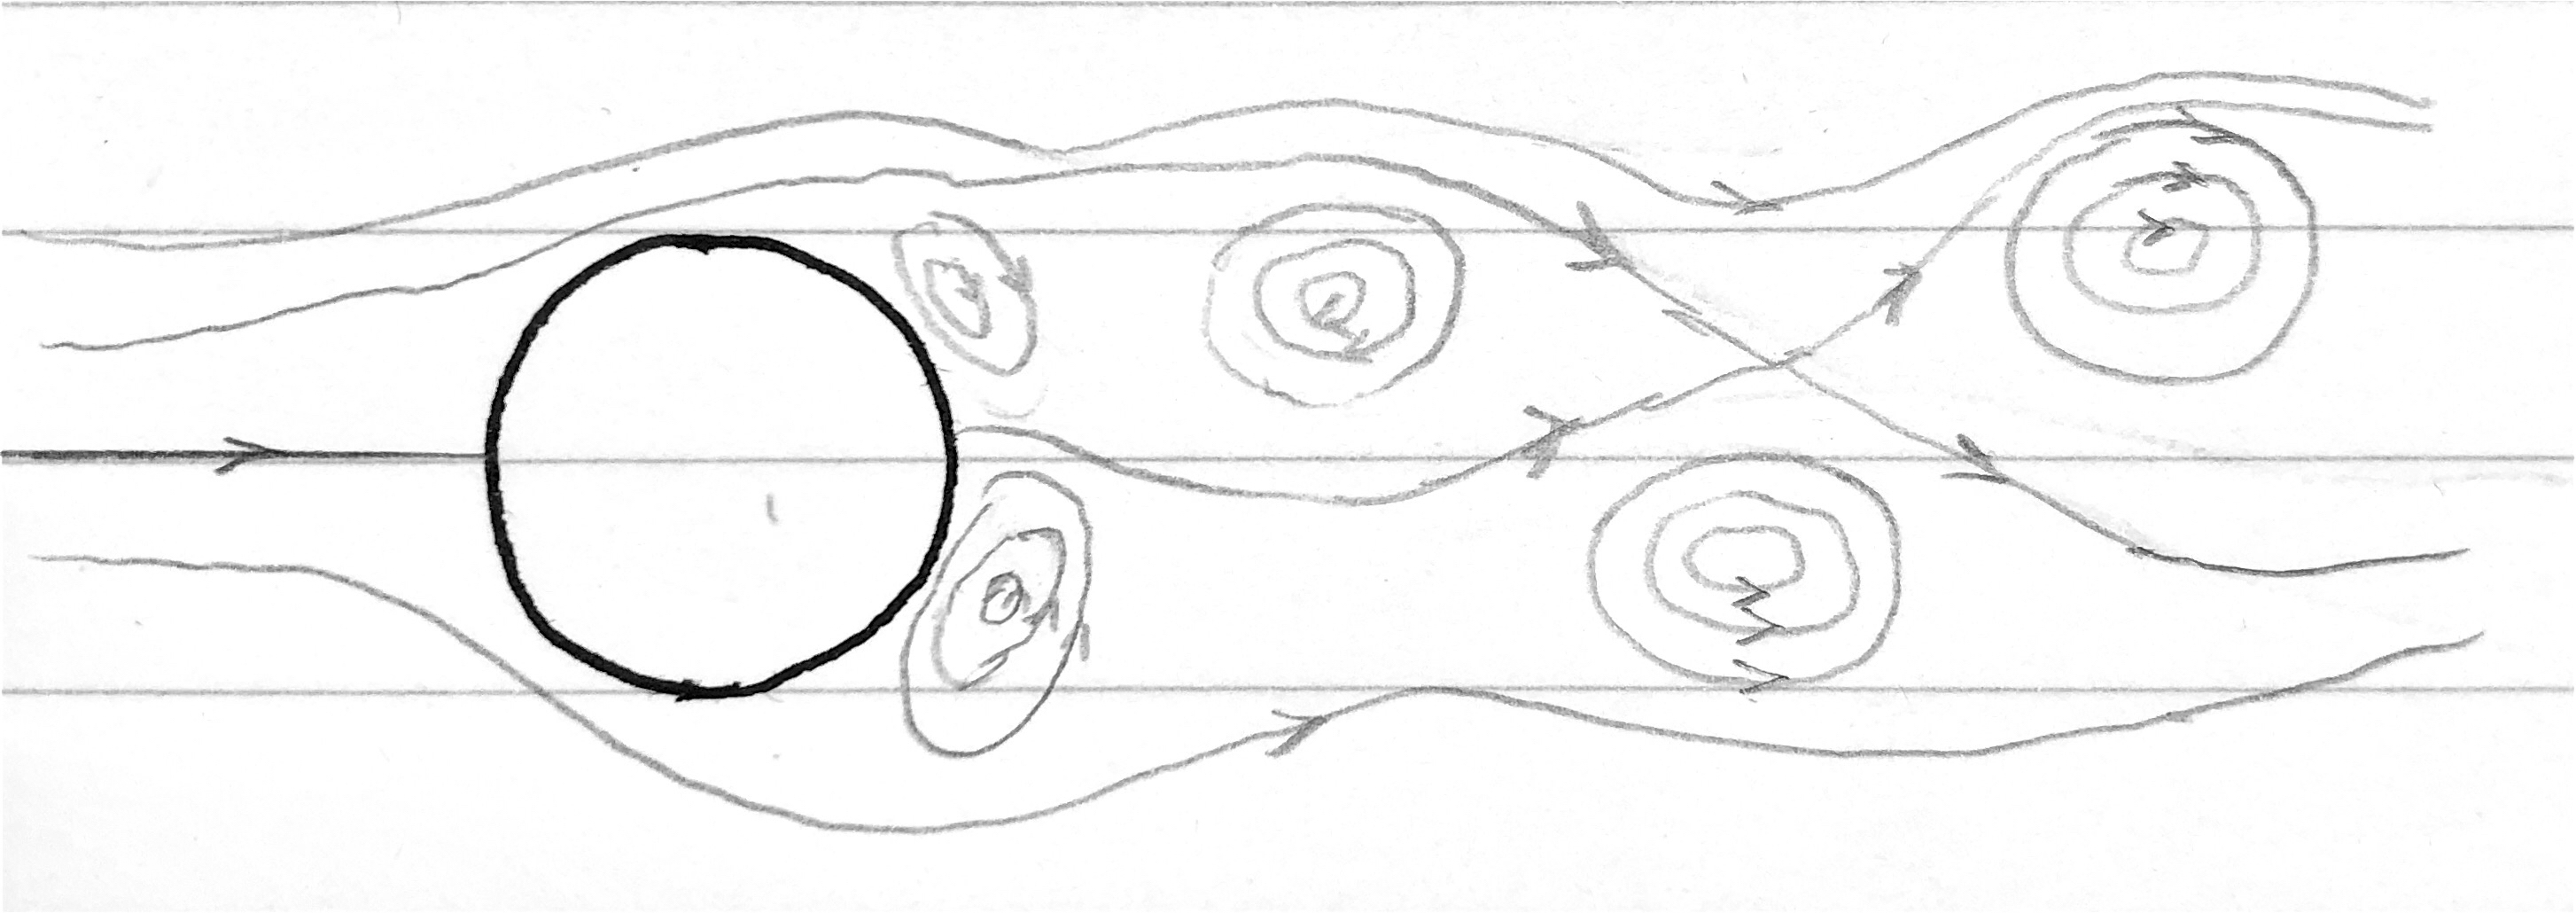
\includegraphics[width=12cm]{streamline.jpg}
	\caption{streamline behind a circular cylinder}
	\label{fig:streamline}
\end{figure}

\section{}

\subsection{}

For any vector $\bm{a}$,
\begin{equation}
	\nabla \cdot \nabla \times \bm{a} = 0,
\end{equation}
so
\begin{equation}
	\nabla \cdot \bm{u} = \nabla \cdot [\lambda \nabla \times(\psi \boldsymbol{r})+\nabla \times \nabla \times(\psi \boldsymbol{r})] = 0.
\end{equation}
For steady fluid,
\begin{equation}
	\frac{\partial \bm{u}}{\partial t} = 0,
\end{equation}
so
\begin{equation}
	\nabla \times \left[ \frac{\partial \bm{u}}{\partial t} + (\bm{u} \cdot \nabla)\bm{u} \right] = \nabla \times \left[ (\bm{u} \cdot \nabla)\bm{u} \right] = 0,
\end{equation}

which means $\bm{u}$ satisfies the steady Euler equation.\qed

\subsection{}



\section{}

Because
\begin{equation}
	\begin{split}
		\bm{n} \cdot \mathbb{B} =\  & n_i \bm{e}_i \cdot (\partial_j u_j \bm{e}_k \bm{e}_k -  \partial_j u_k \bm{e}_k \bm{e}_j) \\
		=\  & n_i \bm{e}_i \cdot \partial_j u_j \bm{e}_k \bm{e}_k - n_i \bm{e}_i \cdot \partial_j u_k \bm{e}_k \bm{e}_j\\
		=\  & n_i \partial_j u_j \bm{e}_i - n_i \partial_j u_i \bm{e}_j
	\end{split}
\end{equation}
and
\begin{equation}
	\begin{split}
		-(\boldsymbol{n} \times \nabla) \times \boldsymbol{u} =\  & - (\bm{e}_i n_j \partial_k \varepsilon_{ijk}) \times \bm{u}\\
		=\  & n_j \partial_k \varepsilon_{njk} u_m \bm{e}_p \varepsilon_{pnm}\\
		=\  & (\delta_{jp}\delta_{km}-\delta_{jm}\delta_{kp}) n_j \partial_k u_m \bm{e}_p\\
		=\  & n_j \partial_k u_k \bm{e}_j - n_j \partial_k u_j \bm{e}_k\\
		=\  & n_i \partial_j u_j \bm{e}_i - n_i \partial_j u_i \bm{e}_j,
	\end{split}
\end{equation}

\begin{equation}
	\boldsymbol{n} \cdot \mathbb{B}=-(\boldsymbol{n} \times \nabla) \times \boldsymbol{u}.\qed
\end{equation}

\section{}

\begin{equation}
	\begin{split}
		\bm{F}\cdot \bm{U} = & - \oiint_{\partial B} \bm{t}\cdot \bm{U} \dif S\\
		= & - \oiint_{\partial B} \bm{t}\cdot \bm{u} \dif S\\
		= & - \oiint_{\partial B} \bm{n}\cdot(\bm{T}\cdot \bm{u}) \dif S\\
		= & - \int_{V} \nabla \cdot (\bm{T}\cdot \bm{u}) \dif V + \oiint_{\Sigma} \bm{t} \cdot \bm{U} \dif S\\
		= & \int p \theta \dif V - \int \Phi \dif V
	\end{split}
\end{equation}













\nocite{*}

\bibliographystyle{plain}
\phantomsection

\addcontentsline{toc}{section}{参考文献} %向目录中添加条目,以章的名义
\bibliography{homework}

\end{document}
